\documentclass{standalone}
\usepackage{tikz}
\begin{document}

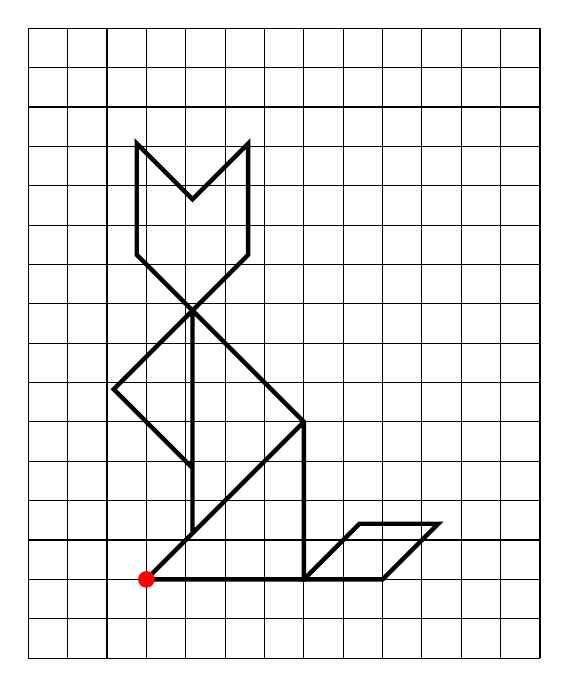
\begin{tikzpicture}[x=1cm,y=1cm]
\draw[step=5mm] (-1.5,-1) grid (5,7);
\draw[ultra thick] ({1-1*sqrt(2)}, {1+1*sqrt(2)}) -- ({2-1*sqrt(2)}, {2+1*sqrt(2)}) -- ({2-3/2*sqrt(2)}, {2+3/2*sqrt(2)}) -- ({2-3/2*sqrt(2)}, {2+5/2*sqrt(2)}) -- ({2-1*sqrt(2)}, {2+2*sqrt(2)}) -- ({2-1/2*sqrt(2)}, {2+5/2*sqrt(2)}) -- ({2-1/2*sqrt(2)}, {2+3/2*sqrt(2)}) -- ({2-1*sqrt(2)}, {2+1*sqrt(2)}) -- ({2-1*sqrt(2)}, {2-1*sqrt(2)}) -- ({2}, {2}) -- ({0}, {0}) -- ({2}, {0}) -- ({2}, {2}) -- ({2-1*sqrt(2)}, {2+1*sqrt(2)}) -- ({2-1*sqrt(2)}, {1*sqrt(2)}) -- ({1-1*sqrt(2)}, {1+1*sqrt(2)}) -- cycle;
\draw[ultra thick] ({2}, {0}) -- ({2+1/2*sqrt(2)}, {1/2*sqrt(2)}) -- ({3+1/2*sqrt(2)}, {1/2*sqrt(2)}) -- ({3}, {0}) -- ({2}, {0}) -- cycle;
\fill[red] (0,0) circle (3pt);
\end{tikzpicture}

\end{document}